% BTP final report -- ISAC-NET
% Compile: pdflatex main && pdflatex main   (or latexmk -pdf main)
% Works on Overleaf as-is (upload this folder with figures/).
\documentclass[11pt,a4paper]{article}

\usepackage[a4paper,margin=1in]{geometry}
\usepackage[T1]{fontenc}
\usepackage{lmodern}
\usepackage{amsmath,amssymb,bm}
\usepackage{graphicx}
\usepackage{booktabs}
\usepackage{array}
\usepackage{tabularx}
\usepackage{caption}
\usepackage{enumitem}
\usepackage{float}
\usepackage[hidelinks]{hyperref}
\pdfstringdefDisableCommands{\def\ensuremath#1{#1}}

\graphicspath{{figures/}}
\captionsetup{font=small,labelfont=bf}
\setlist{itemsep=2pt,topsep=4pt}
\renewcommand{\arraystretch}{1.15}

% ---------- personal details: EDIT THESE ----------
\newcommand{\studentname}{Kushal Dornahalli}       % check spelling
\newcommand{\rollno}{ROLL NO}                      % e.g. 230 1xx xxx
\newcommand{\department}{Department of Electronics and Electrical Engineering} % check
\newcommand{\supervisor}{Prof.\ SUPERVISOR NAME}
\newcommand{\reportdate}{November 2026}
% --------------------------------------------------

\newcommand{\sci}[2]{\ensuremath{#1\times10^{#2}}}
\newcommand{\BH}{\mathbf{H}}
\newcommand{\BX}{\mathbf{X}}
\newcommand{\BY}{\mathbf{Y}}
\newcommand{\BZ}{\mathbf{Z}}

\begin{document}

% ================= TITLE BLOCK (same layout as previous BTP reports) =================
\begin{center}
  {\Large Robust Deep-Unfolded Receivers for Integrated\\[2pt] Passive Sensing and Communication\par}
  \vspace{10pt}
  {\large \studentname\ (\rollno)\par}
  \vspace{4pt}
  \department\par
  Indian Institute of Technology, Guwahati\par
  \vspace{4pt}
  B.Tech Project (7th semester) \quad Supervisor: \supervisor\par
  \vspace{4pt}
  \reportdate
\end{center}

\vspace{6pt}
\begin{abstract}
\noindent In integrated passive sensing and communication (IPSAC), a single receiver must decode the transmitted data and estimate the range and velocity of targets from the same received signal, without knowing the data in advance. ISAC-NET~\cite{isacnet} solves this with an iterative algorithm that alternates symbol detection, passive sensing and channel reconstruction, and unfolds it into a network whose 25 step-size parameters are learned from data.

This project reproduces ISAC-NET end to end at the paper's full simulation size (256 OFDM symbols $\times$ 1024 subcarriers, $8\times 8$ antennas, three targets) in Python and PyTorch, together with the LS, D-AMP and 2D-DFT baselines. Learning the parameters lowers the bit error rate (BER) by 4--19$\times$ compared with the hand-set algorithm, both under our SNR convention and under the paper's own setup, which confirms the paper's main claim.

The reproduction also exposes three limitations the paper does not report. First, training a separate parameter set for each SNR, as the paper does, is brittle: at 15--20~dB a few frames fail completely (BER $\approx 0.5$) and make the average worse than the untrained algorithm. Second, the learned parameters transfer only partly to target layouts not seen in training, where the gain falls from 4--11$\times$ to 3--5$\times$. Third, the same algorithm with four inner iterations per layer reaches perfect-channel BER without any learning, so the benefit of unfolding lies in lower cost rather than higher accuracy. As a first extension, a single parameter set trained on randomly drawn SNR and clutter is never worse than the clean-trained one under clutter. These findings motivate the proposed research direction for the next semester: robust, SNR-adaptive training of deep-unfolded ISAC receivers, with generalisation of multi-target sensing across target placement and count as a second direction.
\end{abstract}

\newpage
\tableofcontents
\newpage

% =====================================================================
\section{Introduction}
Integrated sensing and communication (ISAC) lets one radio system share spectrum and hardware between data transmission and target sensing, and is a candidate feature of 6G networks~\cite{isacnet,zhang2022}. In \emph{active} (monostatic) sensing the receiver sits next to the transmitter and knows the transmitted waveform. In \emph{passive} (bistatic) sensing the sensing receiver is a communication receiver at another site. It avoids full-duplex self-interference, but it does not know the data symbols, so it must decode them before it can use them as a sensing reference.

Sensing from the pilots alone wastes most of the frame, since pilots fill only 1 of every 14 OFDM symbols. Sensing from the data needs correctly decoded symbols, and decoding errors corrupt the sensing estimate, which in turn corrupts the channel used for decoding. ISAC-NET~\cite{isacnet} handles this loop jointly. Its iterative algorithm (Alg.~3 of~\cite{isacnet}) alternates improved D-AMP detection, 2D-DFT range--Doppler sensing on the detected symbols, and channel reconstruction from the sensed targets. Because the result depends on five hand-set parameters per iteration, the authors unfold the iterations into network layers and learn those parameters, a form of model-driven deep learning known as deep unfolding~\cite{oampnet}.

\subsection{Objectives}
This project had two aims: to reproduce ISAC-NET faithfully enough to test its claims, and to find where its approach is weak, as the basis for research in the next semester.

\subsection{Contributions}
\begin{enumerate}
  \item An open Python/PyTorch implementation of the full system model, three baselines, Alg.~3 and ISAC-NET at the paper's Table~III size, with unit tests (\url{https://github.com/Kushal2oo4/isac-net}).
  \item A list of points where the paper is ambiguous or inconsistent, the choice made for each, and a quantitative explanation of why our figures differ from the published ones.
  \item A reproduction of the paper's main claim: learning lowers BER by 4--19$\times$ compared with the hand-set algorithm, under both our setup and the paper's.
  \item Three findings beyond the paper: per-SNR training is brittle; the learned parameters transfer only partly to unseen target layouts; and a converged hand-set algorithm already reaches perfect-channel BER.
  \item A first extension towards robustness: clutter scatterers in the channel model and a single parameter set trained over random SNR and clutter.
\end{enumerate}

Section~\ref{sec:background} reviews background, Section~\ref{sec:model} gives the system model, Section~\ref{sec:algos} the algorithms and Section~\ref{sec:impl} the implementation and setup. Section~\ref{sec:results} presents the results, Section~\ref{sec:future} the proposed research directions, and Section~\ref{sec:conclusion} concludes.

% =====================================================================
\section{Background}\label{sec:background}
\subsection{OFDM radar sensing}
With OFDM, the radar channel can be read directly from the data: dividing each received resource element by the transmitted symbol removes the modulation, leaving a matrix whose phase rotates with delay across subcarriers and with Doppler across symbols. An inverse DFT over subcarriers and a DFT over symbols then give a range--velocity map, whose peaks are the targets~\cite{sturm2011}. This works only when the transmitted symbols are known, which is why passive sensing depends on correct detection.

\subsection{Deep unfolding}
An iterative algorithm with a fixed number of iterations can be written as a feed-forward network, one layer per iteration. Its hand-set parameters (step sizes, damping factors, thresholds) become trainable weights, while the structure of the algorithm is kept. The result needs far fewer parameters and training samples than a black-box network and stays interpretable. OAMP-Net2~\cite{oampnet} applies this to MIMO detection and is one of the baselines in~\cite{isacnet}.

\subsection{ISAC-NET}
ISAC-NET~\cite{isacnet} combines the two: it unfolds an iterative receiver that detects symbols, senses targets from the detected symbols, and rebuilds the channel from the targets. It reports BER close to OAMP-Net2 and better than a model-free network (TPG), with range and velocity NMSE close to the Cram\'er--Rao bound at high SNR. Its learned parameters are trained offline and stored separately for each SNR.

% =====================================================================
\section{System Model}\label{sec:model}
A base station with $N_t$ antennas sends an OFDM frame of $M$ symbols $\times$ $N$ subcarriers. A receiver with $N_r$ antennas at another site decodes the data and senses $L_p$ point targets from their echoes, following~\cite[Sec.~II]{isacnet}.

\subsection{Transmitted frame}
The same symbol $x(m,n)$ is sent on every transmit antenna, so the transmit vector is $\mathbf{x}(m,n)=[x(m,n),\dots,x(m,n)]^T$. One of every 14 OFDM symbols is a known QPSK pilot; the rest carry 16-QAM data.

\subsection{Channel}
Each target reflects the signal once. Path $l$ has length $r_l=r_{1,l}+r_{2,l}$ (transmitter to target plus target to receiver), delay $\tau_l=r_l/c$ and Doppler shift $f_{d,l}=v_l f_c/c$. Its channel at symbol $m$ and subcarrier $n$ is
\begin{equation}
  \tilde{\BH}_l(m,n)=\sqrt{F_l}\,f_l\,e^{-j2\pi(f_c+n\Delta f)\tau_l}\,e^{j2\pi f_{d,l} m T}\,\mathbf{d}_r(\theta_r^l)\,\mathbf{d}_t^H(\theta_t^l),
\end{equation}
where $\mathbf{d}_t$ and $\mathbf{d}_r$ are the transmit and receive steering vectors, $f_l$ is small-scale (Weibull) fading, and
\begin{equation}
  F_l=\frac{\lambda^2\sigma_l}{(4\pi)^3\,(r_{1,l}\,r_{2,l})^2}
\end{equation}
is the bistatic path loss with radar cross-section $\sigma_l$. The received vector is
\begin{equation}
  \mathbf{y}(m,n)=\sum_{l=0}^{L_p-1}\tilde{\BH}_l(m,n)\,\mathbf{x}(m,n)+\mathbf{z}(m,n)
\end{equation}
with white Gaussian noise $\mathbf{z}(m,n)$. Stacking all $MN$ resource elements gives~\cite[eq.~(9)]{isacnet}
\begin{equation}
  \BY=\sum_{l=0}^{L_p-1}\BH_a^l\,\BX\,\BH_\varphi^l+\BZ,\qquad
  \BH_a^l=\sqrt{F_l}\,f_l\,\mathbf{d}_r\mathbf{d}_t^H,\qquad
  \BH_\varphi^l=\operatorname{diag}\!\big(e^{-j2\pi(f_c+n\Delta f)\tau_l}e^{j2\pi f_{d,l}mT}\big).
\end{equation}
$\BY$ is $N_r\times MN$, $\BX$ is $N_t\times MN$ with identical rows, $\BH_a^l$ holds the gain and angles of path $l$, and the diagonal matrix $\BH_\varphi^l$ holds its delay and Doppler phases.

\subsection{Problem formulation}
The receiver jointly estimates the data and the target parameters by least squares~\cite[eq.~(18)]{isacnet}:
\begin{equation}
  \min_{\BX,\,\mathbf{r},\,\mathbf{v}}\ \Big\|\BY-\sum_l\BH_a^l\BX\BH_\varphi^l\Big\|^2
  \quad\text{s.t.}\quad\{\BH_a^l,\BH_\varphi^l\}=F_3(\mathbf{r},\mathbf{v}),
\end{equation}
where $F_3$ rebuilds the channel from the estimated ranges $\mathbf{r}$ and velocities $\mathbf{v}$. Since $\BX$ enters through the channel and the channel depends on the targets, the problem is solved by alternating over $\BX$, $(\mathbf{r},\mathbf{v})$ and the channel.

\subsection{Resolution}
With bandwidth $B=N\Delta f\approx 123$~MHz, the range bin is $c/B\approx 2.4$~m. With frame duration $MT\approx 2.66$~ms at $f_c=4$~GHz, the velocity bin is $c/(TMf_c)\approx 28$~m/s. The test targets move at 5, 10 and 15~m/s, so they cannot be separated in velocity, only in range.

% =====================================================================
\section{Algorithms}\label{sec:algos}
All receivers start from the pilot symbols, which give a least-squares (LS) channel estimate and a coarse range--Doppler map. They differ in how they use the data symbols.

\subsection{Baselines}
\begin{itemize}
  \item \textbf{LS + MAP.} The channel is estimated by LS on the pilots, and each data symbol is detected by a maximum a posteriori (MAP) decision.
  \item \textbf{Improved D-AMP (Alg.~1 of~\cite{isacnet}).} Starting from $\BX=\BZ=\mathbf{0}$, it repeats a signal update and a residual update:
  \begin{align}
    \BX_d^{k+1}&=\eta_1^k\BX_d^k+\sum_l(\hat{\BH}_a^l)^H\BZ_d^k(\hat{\BH}_\varphi^l)^H,\\
    \BZ_d^{k+1}&=\eta_2^k\BZ_d^k+\BY_d-\sum_l\hat{\BH}_a^l\BX_d^k\hat{\BH}_\varphi^l.
  \end{align}
  \item \textbf{2D-DFT sensing~\cite{sturm2011}.} The received symbols are divided element-wise by the transmitted (or detected) symbols, $S(m,n)=y(m,n)/x(m,n)$. An IDFT over subcarriers gives range and a DFT over symbols gives velocity, each zero-padded $10\times$. Peaks are extracted one at a time.
  \item \textbf{Channel reconstruction (Alg.~2 of~\cite{isacnet}).} The channel of each path is rebuilt from its estimated range and velocity through $\BH_\varphi$ (delay and Doppler phases) and $\BH_a$ (gain and angles).
\end{itemize}

\subsection{Alg.~3: iterative ISAC signal processing}
Iteration $k$ uses five parameters $\Omega_k=(\eta_1,\eta_2,\eta_3,\eta_4,\eta_5)$:
\begin{enumerate}
  \item \textbf{Detect:} one D-AMP signal and residual update with $\eta_1$ and $\eta_2$, using the current channel.
  \item \textbf{Sense:} 2D-DFT on the detected symbols; peaks above the threshold $\eta_3$ are taken one by one as targets.
  \item \textbf{Blend targets:} $(\mathbf{r},\mathbf{v})\leftarrow\eta_4\cdot(\mathbf{r},\mathbf{v})_{\text{old}}+(\mathbf{r},\mathbf{v})_{\text{new}}$.
  \item \textbf{Rebuild the channel:} $\BH_{\text{new}}=F_3(\mathbf{r},\mathbf{v})$.
  \item \textbf{Blend the channel:} $\BH\leftarrow\eta_5\cdot\BH_{\text{old}}+\BH_{\text{new}}$, then return to step 1.
\end{enumerate}
We study two variants: the \emph{literal} one, with one D-AMP update per iteration as written in~\cite{isacnet}, and a \emph{converging} one, with four D-AMP updates per iteration.

\subsection{ISAC-NET}
ISAC-NET unfolds $K$ iterations of Alg.~3 into $K$ layers with the same structure and separate trainable $\Omega_k$, so $5K$ parameters in total (25 for $K=5$). The paper trains them in TensorFlow with batch 128, 500 epochs and learning rate 0.001, and stores one parameter set per SNR~\cite[Sec.~IV-B]{isacnet}. Our implementation uses PyTorch and the loss
\begin{equation}
  \mathcal{L}=\frac{1}{|\mathcal{D}|}\sum_{(m,n)\in\mathcal{D}}|\hat{x}(m,n)-x(m,n)|^2+\lambda\big(\mathrm{NMSE}_r+\mathrm{NMSE}_v\big),\qquad\lambda=1,
\end{equation}
where $\mathcal{D}$ is the set of data resource elements (unit-power 16-QAM) and each NMSE is averaged over the targets, a missed target counting as NMSE~1. Training uses Adam, gradient-norm clipping, a cosine learning-rate schedule and a box constraint on each $\eta$. It keeps the parameters with the lowest loss on fixed validation frames, starting from the hand-set values, so a trained network is never worse than Alg.~3 on those frames.

We compare two training schemes:
\begin{itemize}
  \item \textbf{Per-SNR}, as in~\cite{isacnet}: one training run, and one stored $\Omega$, per SNR.
  \item \textbf{Joint}: one $\Omega$ for all SNRs, where every training and validation frame draws its SNR at random from the training range.
\end{itemize}

% =====================================================================
\section{Implementation and Simulation Setup}\label{sec:impl}
All results use the paper's Table~III parameters at full size (Table~\ref{tab:params}); nothing is scaled down.

\begin{table}[H]
\centering
\begin{tabular}{ll}
\toprule
Parameter & Value \\
\midrule
Carrier frequency $f_c$ & 4 GHz \\
Subcarrier spacing $\Delta f$ & 120 kHz \\
OFDM symbols $M$ / subcarriers $N$ & 256 / 1024 \\
DFT / IDFT points $M_I$ / $N_I$ & 2560 / 10240 ($10\times$ zero padding) \\
Symbol time $T$ ($T_p+T_c$) & 10.38 \textmu s (8.3 + 2.08 \textmu s) \\
Antennas $N_t=N_r$ & 8 \\
Modulation, pilot ratio & 16-QAM, 1/14 \\
Targets & 3, at 10/50/100 m and 5/10/15 m/s, RCS 1 m$^2$ \\
Path loss & Physical bistatic (targets differ by about 40 dB) \\
\bottomrule
\end{tabular}
\caption{Simulation parameters (Table III of~\cite{isacnet}).}
\label{tab:params}
\end{table}

\subsection{Data generation}
The paper generates its data sets in MATLAB. We simulate the same model in Python with NumPy: the transmit frame from eq.~(1), the received signal from eq.~(6), and the channel from eqs.~(10), (13) and (14) of~\cite{isacnet}. The tool does not change the model, but the random draws differ, so curves can match in shape but not point by point.
\begin{itemize}
  \item \textbf{Fresh data every step.} Every training step draws new symbols, channels and noise, instead of a fixed data set split 95\%/5\%. Validation and test frames come from separate random seeds.
  \item \textbf{Fixed pilots.} The same QPSK pilot sequence is used in every frame, as the paper requires.
  \item \textbf{Unstated channel details.} The paper does not give target angles or the exact gain model. We draw AoD and AoA uniformly in $\pm60^\circ$, use Weibull small-scale fading, and use physical path loss.
  \item \textbf{Fixed targets.} Training uses the targets of Table~\ref{tab:params}, with angles, fading and noise changing between frames. Section~\ref{sec:paper-lr} tests the trained network on randomly placed targets.
\end{itemize}

\subsection{Interpretation choices}
The paper leaves several steps open or states them inconsistently. The choices in Table~\ref{tab:choices} were needed for the algorithm to work as described; the repository README lists all of them.

\begin{table}[H]
\centering\small
\begin{tabularx}{\textwidth}{>{\raggedright\arraybackslash}X>{\raggedright\arraybackslash}X>{\raggedright\arraybackslash}X}
\toprule
Point in~\cite{isacnet} & Our choice & Effect \\
\midrule
Alg.~3 runs one D-AMP update per iteration, far from converged after 5 iterations & Two variants: literal (1 update) and converging (4 updates) & The converging variant reaches perfect-channel BER without learning \\
Residual update (24) uses $\BX^k$, so $\eta_1=1,\eta_2=0$ oscillates for any step size & Conjugate transpose in (23), step size $0.5/\|h\|^2$ & Literal BER rises from layer 2 to 3; learned $\eta_1\approx0.9$ acts as damping \\
Peaks removed by plain subtraction & Each peak refined off-grid and all gains re-fitted jointly by LS & Without it, residues of the 10 m target hide the 100 m target \\
$\eta_3$ is a hard threshold & Sigmoid gate on peak height & Gives $\eta_3$ a gradient \\
Blends read ``$\eta\cdot$old + new'' & Convex blends $\eta\cdot$old $+(1-\eta)\cdot$new & Keeps $r$, $v$ and $\BH$ unbiased for any $\eta$ \\
Search range not stated & $r\le200$ m, $|v|\le50$ m/s (``search window'') & Avoids spurious far peaks; Section~\ref{sec:paper-setup} tests without it \\
$\BH_\varphi$ is diagonal, yet complexity is given as $O(L_pN_tN_r(MN)^2)$ & Applied element-wise & A layer costs $O(L_pN_tN_rMN)$ \\
SNR definition not stated & Per receive antenna, or after combining the $N_r$ antennas & The two differ by 9 dB; Section~\ref{sec:paper-setup} \\
\bottomrule
\end{tabularx}
\caption{Main interpretation choices.}
\label{tab:choices}
\end{table}

\subsection{Training runs}
\begin{table}[H]
\centering\footnotesize
\setlength{\tabcolsep}{3.5pt}
\begin{tabular}{llcllcc}
\toprule
Run & SNR definition & Layers & Training SNRs & Steps $\times$ batch & LR & Val.\ frames \\
\midrule
A1, per-SNR & Per antenna & 5 & 0--25 dB, one run each & $300\times4$ & 0.01 & 16 per SNR \\
A2, joint & Per antenna & 5 & 0--25 dB, random per frame & $300\times8$ & 0.01 & 48 \\
B1, joint & After combining & 10 & 0--40 dB & $200\times8$ & 0.01 & 48 \\
B2, joint & After combining & 5 & 0--25 dB & $200\times8$ & 0.002 & 48 \\
\bottomrule
\end{tabular}
\caption{Training runs. All use Adam, gradient clipping at 1.0 and 200 test frames per SNR. Runs B also hold the first pilot's LS estimate for the whole frame, as the paper's ``conventional'' receiver appears to.}
\label{tab:runs}
\end{table}

Everything ran on the CPU of an Apple M2 Pro (Apple MPS lacks complex linear solves). A training run takes 1--4.5~h, and a 200-frame evaluation over 11 SNRs about 1~h. Training is much shorter than the paper's 500 epochs $\times$ batch 128, but with only 25 parameters the validation loss stops improving within 100--200 steps.

% =====================================================================
\section{Results}\label{sec:results}
Learning the parameters of the literal algorithm improves both communication and sensing, but only with joint training, and a converged hand-set algorithm remains the best receiver. Sections~\ref{sec:comm}--\ref{sec:layers} use run A (SNR per receive antenna); Sections~\ref{sec:paper-setup}--\ref{sec:paper-lr} use the paper's setup, and Section~\ref{sec:clutter} adds clutter.

\subsection{Communication (cf.\ Fig.~9 of~\cite{isacnet})}\label{sec:comm}
\begin{figure}[H]
\centering
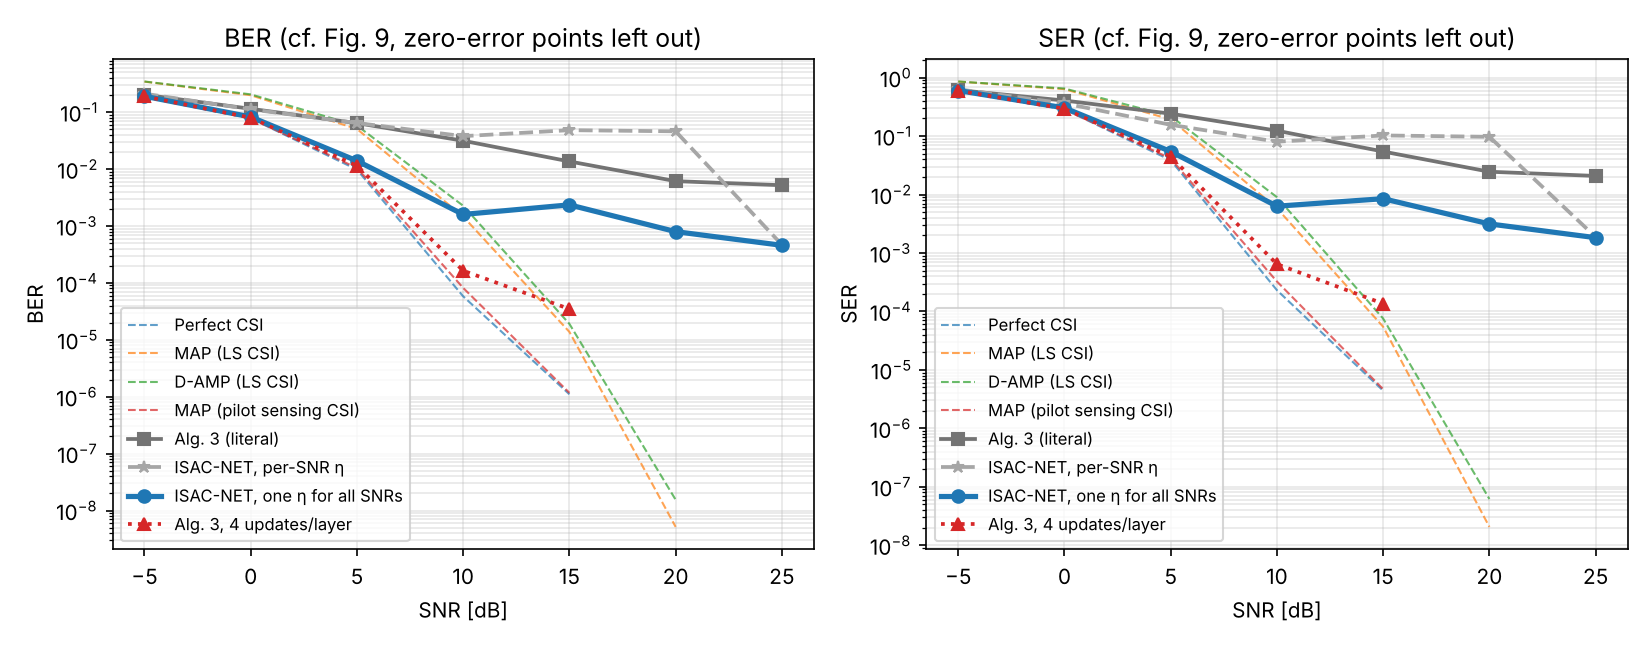
\includegraphics[width=\textwidth]{final_fig9.png}
\caption{BER (left) and SER (right) versus SNR, 200 frames per SNR. Thin dashed lines are baselines; points with zero errors are left out.}
\label{fig:ber}
\end{figure}

\begin{table}[H]
\centering\small
\setlength{\tabcolsep}{3.5pt}
\begin{tabular}{lcccccc}
\toprule
SNR (dB) & 0 & 5 & 10 & 15 & 20 & 25 \\
\midrule
Alg.~3, literal & \sci{1.1}{-1} & \sci{6.4}{-2} & \sci{3.1}{-2} & \sci{1.4}{-2} & \sci{6.1}{-3} & \sci{5.2}{-3} \\
ISAC-NET, per-SNR (A1) & \sci{1.1}{-1} & \sci{6.5}{-2} & \sci{3.8}{-2} & \sci{4.8}{-2} & \sci{4.6}{-2} & \sci{4.7}{-4} \\
ISAC-NET, joint (A2) & \sci{8.3}{-2} & \sci{1.4}{-2} & \sci{1.6}{-3} & \sci{2.4}{-3} & \sci{8.0}{-4} & \sci{4.6}{-4} \\
Alg.~3, 4 updates per layer & \sci{8.0}{-2} & \sci{1.1}{-2} & \sci{1.6}{-4} & \sci{3.5}{-5} & 0 & 0 \\
Perfect channel + MAP & \sci{7.8}{-2} & \sci{9.8}{-3} & \sci{5.8}{-5} & \sci{1.1}{-6} & 0 & 0 \\
\bottomrule
\end{tabular}
\caption{BER versus SNR, SNR per receive antenna.}
\label{tab:ber}
\end{table}

\begin{itemize}
  \item \textbf{Learning helps the literal algorithm.} Joint training lowers BER $4.6\times$ at 5 dB, $19\times$ at 10 dB, $6\times$ at 15 dB and $8\times$ at 20 dB. This reproduces the paper's main claim.
  \item \textbf{Per-SNR training fails at 15--20 dB.} Its median BER there is about $10^{-5}$ and 0, better than Alg.~3, but 2--6 of 24 test frames fail completely (BER $\approx0.5$) and dominate the mean. With 16 validation frames per SNR, training rarely sees such a frame. The $\Omega$ trained at 25 dB had no failures at 15 and 20 dB, which shows the fault lies in the training, not in the SNR.
  \item \textbf{Convergence matters more than learning.} With four D-AMP updates per layer, the hand-set algorithm stays within a factor 3 of the perfect channel at 10 dB, and training finds nothing better.
  \item \textbf{Pilot-based reconstruction is already strong.} At 0 dB, MAP with the channel rebuilt from pilot sensing (BER \sci{7.84}{-2}) matches the perfect channel (\sci{7.77}{-2}), against 0.20 for LS + MAP.
\end{itemize}

\subsection{Sensing (cf.\ Fig.~10 of~\cite{isacnet})}\label{sec:sensing}
\begin{figure}[H]
\centering
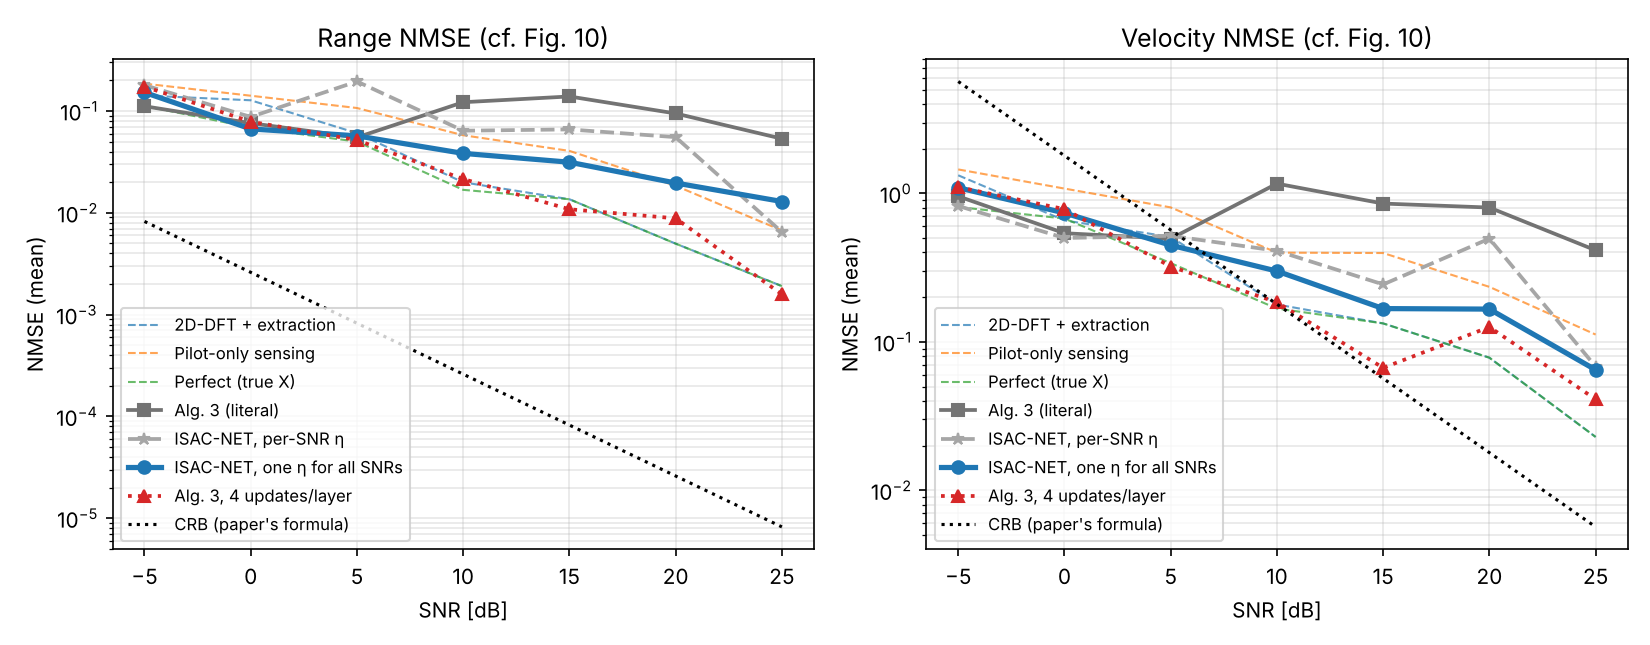
\includegraphics[width=\textwidth]{final_fig10.png}
\caption{Mean range (left) and velocity (right) NMSE versus SNR, with the CRB as drawn in~\cite{isacnet}.}
\label{fig:nmse}
\end{figure}

Joint training lowers range NMSE from \sci{1.2}{-1} to \sci{3.8}{-2} at 10 dB and from \sci{5.3}{-2} to \sci{1.3}{-2} at 25 dB. It lowers velocity NMSE from 1.2 to 0.30 at 10 dB and from 0.41 to 0.065 at 25 dB. At 0 dB the velocity NMSE gets slightly worse (0.54 to 0.74). All methods stay well above the CRB, because the 28 m/s velocity bin is wider than the 5 m/s spacing of the targets; on-grid estimates cannot get much below NMSE $10^{-2}$. Mean NMSE is driven by a few frames with a missed target; the median range NMSE is about $10^{-7}$.

\subsection{Convergence over layers (cf.\ Fig.~8 of~\cite{isacnet})}\label{sec:layers}
\begin{figure}[H]
\centering
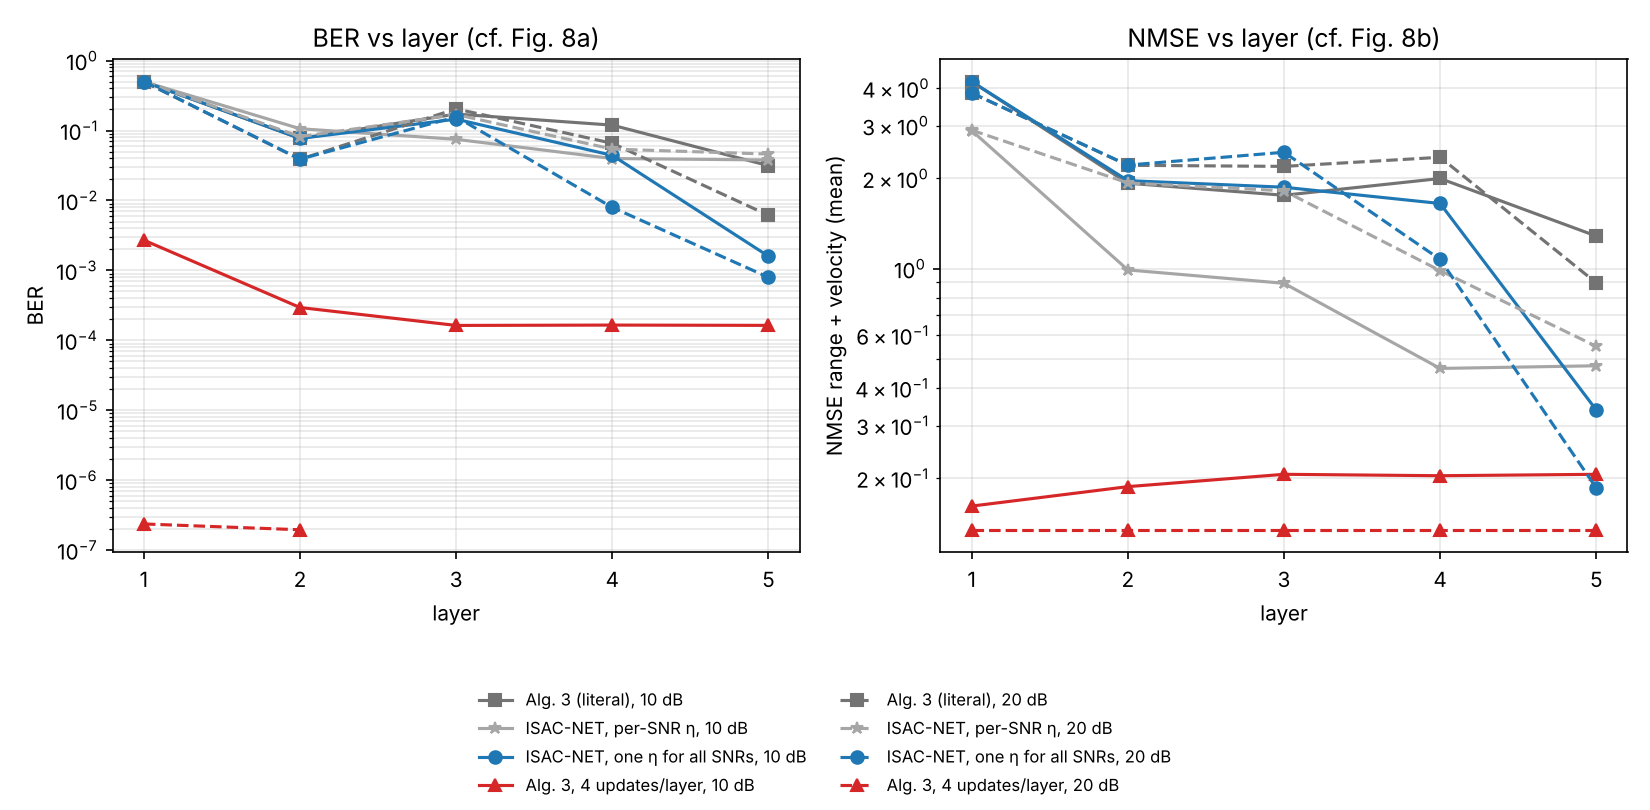
\includegraphics[width=\textwidth]{final_fig8.png}
\caption{BER (left) and range + velocity NMSE (right) after each layer, at 10 dB (solid) and 20 dB (dashed).}
\label{fig:layers}
\end{figure}

Literal Alg.~3 gets worse from layer 2 to layer 3 at every SNR, the oscillation noted in Table~\ref{tab:choices}. Learning does not remove it at layer 3, but it makes layers 4 and 5 converge: at 20 dB, BER falls from \sci{1.5}{-1} at layer 3 to \sci{8.0}{-4} at layer 5, against \sci{6.1}{-3} for Alg.~3. The 4-update variant converges within 2--3 layers.

\subsection{Comparison with the paper's setup}\label{sec:paper-setup}
Our run-A curves have the same shape as the paper's but sit about 9 dB to the left, and our sensing never shows the paper's NMSE of about $10^5$ at low SNR. Table~\ref{tab:diffs} lists the differences and their causes; run B tests the main ones by adopting the paper's choices.

\begin{table}[H]
\centering\small
\begin{tabularx}{\textwidth}{>{\raggedright\arraybackslash}p{3.3cm}>{\raggedright\arraybackslash}p{2.4cm}>{\raggedright\arraybackslash}X>{\raggedright\arraybackslash}p{3.2cm}}
\toprule
Feature of~\cite{isacnet} & Run A & Cause & Tested in run B \\
\midrule
Perfect-channel BER $10^{-5}$ at about 21 dB & At about 12 dB & SNR per antenna vs after combining 8 antennas (9 dB) & Yes: shift disappears \\
``Conventional'' LS + MAP floors at BER 0.1 & No floor & Our LS is interpolated between pilots; \cite{isacnet} likely holds one estimate & Yes: floor of about 0.2 appears \\
NMSE about $10^5$ below a threshold SNR & NMSE at most about 1 & Our 200 m / 50 m/s search window rules out far-off peaks & Yes: without the window, the literal receiver fails \\
Fig.~8 uses 10 layers & 5 layers & Choice of depth & Yes (B1) \\
Velocity NMSE down to $10^{-3}$--$10^{-4}$ & Best \sci{6.5}{-2} & 28 m/s bin vs 5 m/s target spacing & No: needs off-grid estimation \\
CRB line almost flat & CRB falls $10\times$ per 10 dB & Drawn line does not follow~\cite{isacnet}'s own formula $\Delta R/\sqrt{2\,\mathrm{SNR}}$ & No: inherent in~\cite{isacnet} \\
OAMP-Net2 and TPG curves & Not implemented & Out of scope & No \\
\bottomrule
\end{tabularx}
\caption{Differences from the published figures.}
\label{tab:diffs}
\end{table}

\begin{figure}[H]
\centering
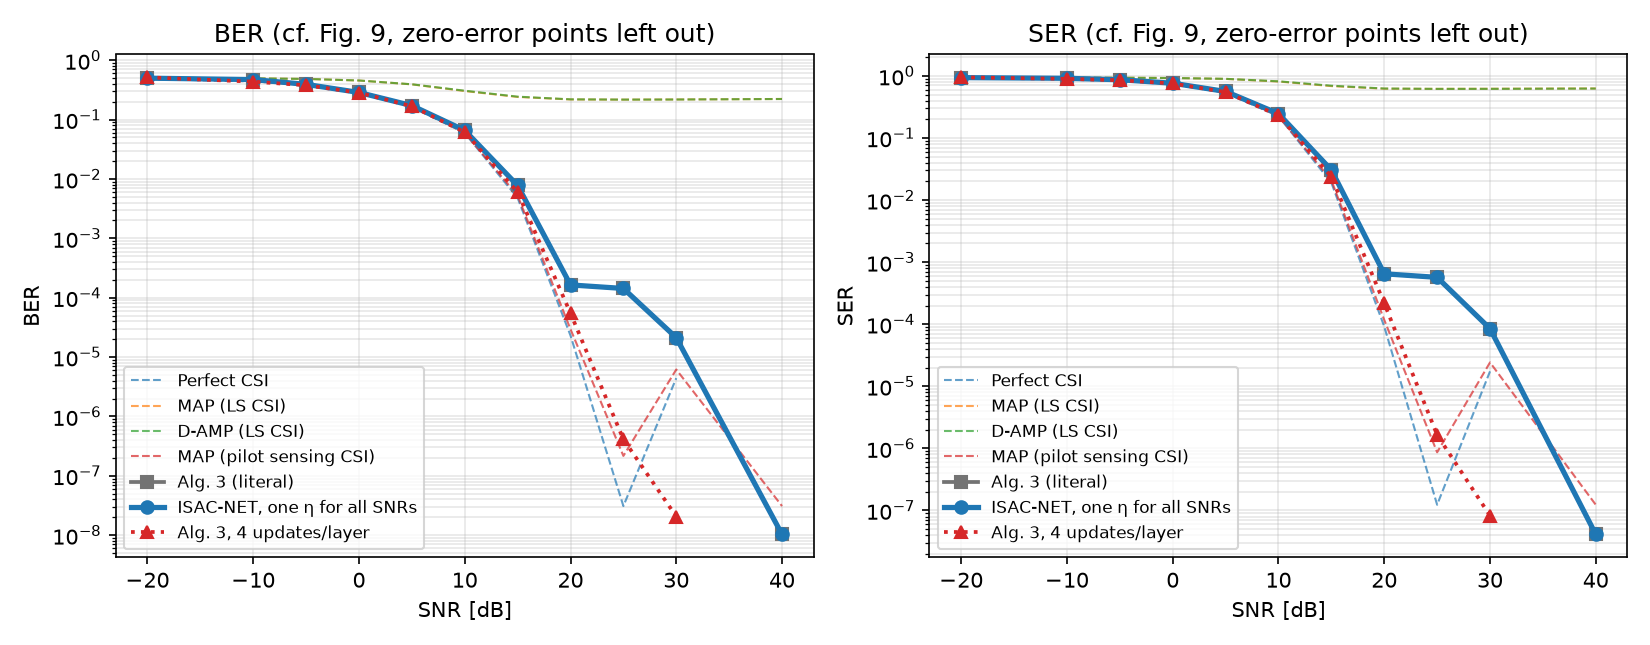
\includegraphics[width=\textwidth]{paper_window_fig9.png}
\caption{BER and SER with SNR measured after combining, 10 layers, hand-set parameters (run B1 setup, with the search window).}
\label{fig:paper-window}
\end{figure}

With SNR measured after combining, the 4-update Alg.~3 reaches BER \sci{5.5}{-5} at 20 dB and follows the perfect-channel curve, which in~\cite{isacnet} reaches $10^{-5}$ at about 21 dB: the 9 dB offset is explained. Holding the first pilot's LS estimate gives LS + MAP and D-AMP a floor of about 0.2, the shape of the paper's ``conventional'' curve. Without the search window, literal Alg.~3 has BER about 0.5 at every SNR, even 40 dB, and velocity NMSE about $4\times10^4$: a wrong velocity peak corrupts the rebuilt channel and ruins detection. The 4-update variant gives about the same BER with or without the window.

Training in run B1 (10 layers, 0--40 dB, learning rate 0.01) diverged. Validation loss rose from 0.666 to 4.87 over 200 steps, so checkpointing kept the hand-set values and the network learned nothing.

\subsection{Retraining at a lower learning rate, and unseen targets}\label{sec:paper-lr}
Run B2 lowered the learning rate to 0.002, closer to the paper's 0.001, with 5 layers and training SNRs of 0--25 dB. A 40-step test confirmed the loss fell before the full run. Over 200 steps the validation loss fell from 1.97 (hand-set) to 0.84 at step 100, then stayed between 0.91 and 1.03.

\begin{figure}[H]
\centering
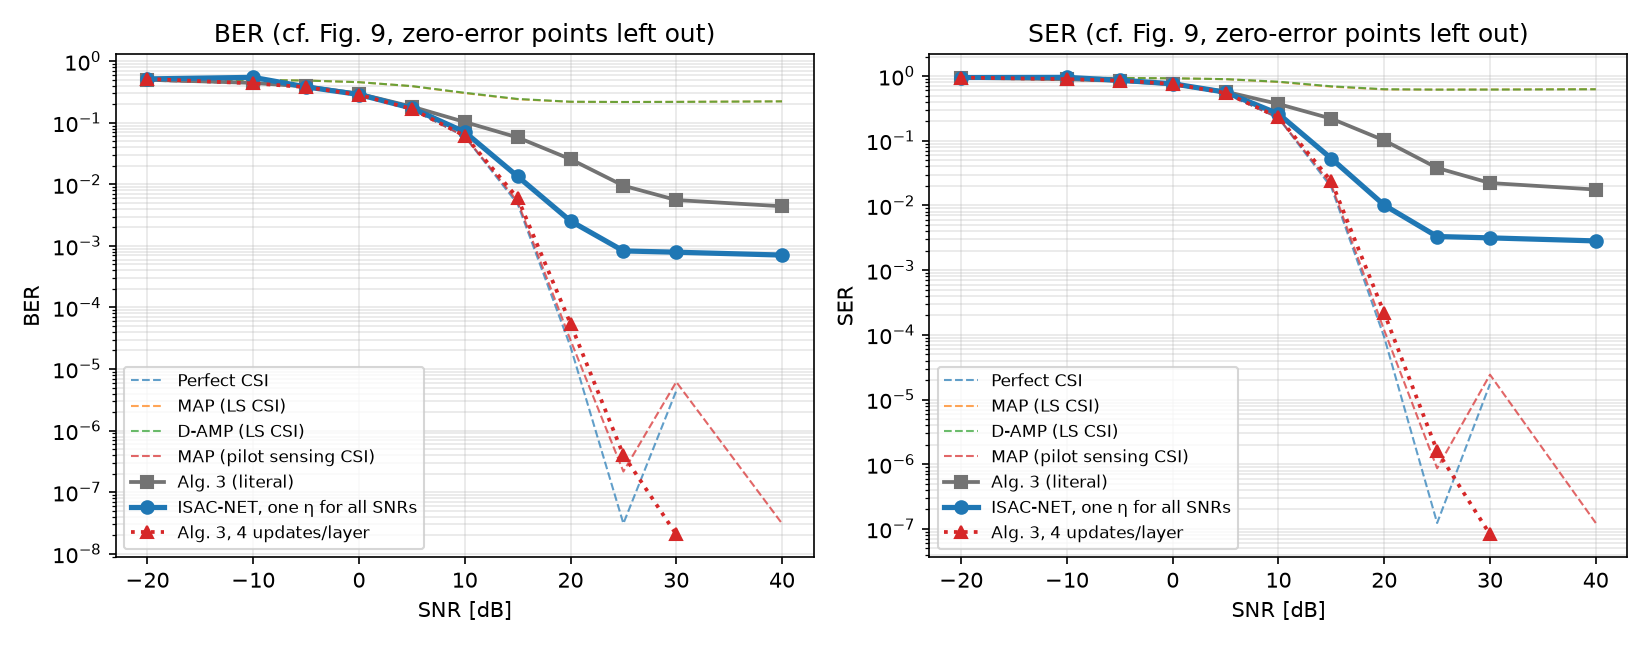
\includegraphics[width=\textwidth]{paper_lr_fig9.png}
\caption{BER and SER under the paper's setup after retraining (run B2, 5 layers, with the search window).}
\label{fig:paper-lr}
\end{figure}

\begin{table}[H]
\centering\small
\setlength{\tabcolsep}{3.5pt}
\begin{tabular}{lccccc}
\toprule
SNR (dB) & 10 & 15 & 20 & 25 & 30 \\
\midrule
Alg.~3, literal & \sci{1.0}{-1} & \sci{5.8}{-2} & \sci{2.6}{-2} & \sci{9.5}{-3} & \sci{5.6}{-3} \\
ISAC-NET, output (layer 5) & \sci{7.1}{-2} & \sci{1.3}{-2} & \sci{2.5}{-3} & \sci{8.3}{-4} & \sci{7.9}{-4} \\
ISAC-NET, layer 4 & \sci{8.3}{-2} & \sci{2.3}{-2} & \sci{1.8}{-3} & \sci{3.1}{-5} & \sci{2.8}{-6} \\
Alg.~3, 4 updates per layer & \sci{6.1}{-2} & \sci{6.0}{-3} & \sci{5.5}{-5} & \sci{4.0}{-7} & \sci{2.1}{-8} \\
\midrule
\emph{Random targets:} Alg.~3, literal & \sci{1.1}{-1} & \sci{6.2}{-2} & \sci{3.5}{-2} & \sci{1.9}{-2} & \sci{1.5}{-2} \\
\emph{Random targets:} ISAC-NET (layer 5) & \sci{7.5}{-2} & \sci{2.2}{-2} & \sci{6.4}{-3} & \sci{4.4}{-3} & \sci{4.4}{-3} \\
\bottomrule
\end{tabular}
\caption{BER under the paper's setup, run B2, with the search window. Random targets: path length 5--150 m (at least 5 m apart), speed 3--30 m/s in either direction, drawn anew per frame and never seen in training.}
\label{tab:paper-lr}
\end{table}

\begin{itemize}
  \item \textbf{Learning helps under the paper's setup too.} ISAC-NET lowers BER 4--11$\times$ compared with literal Alg.~3 at 15--25 dB, and velocity NMSE from 1.1 to 0.20 at 20 dB. Below 5 dB there is little or no gain.
  \item \textbf{The last layer limits high-SNR BER.} Output BER stays near \sci{8}{-4} from 25 to 40 dB, while layer 4 reaches \sci{3.1}{-5} at 25 dB and no errors at 40 dB. The fifth layer undoes part of the convergence, the same oscillation as in Section~\ref{sec:layers}.
  \item \textbf{The gain transfers only partly to unseen targets.} On random target layouts the gain falls to 3--5$\times$, and ISAC-NET levels off at \sci{4.4}{-3} instead of \sci{8}{-4}. The learned $\Omega$ is partly tuned to the training scenario.
  \item \textbf{Training does not repair the missing window.} Without it, trained ISAC-NET still has BER above 0.4 at every SNR.
  \item \textbf{The converged algorithm stays best.} The 4-update Alg.~3 reaches \sci{5.5}{-5} at 20 dB, against \sci{2.5}{-3} for ISAC-NET.
\end{itemize}

\subsection{Extension: clutter and one model for all conditions}\label{sec:clutter}
One $\eta$ trained on randomly drawn SNR and clutter replaces per-SNR training: it is never worse than the clean-trained $\eta$ and lowers BER at 15--25 dB in every test condition. Following~\cite{clutter}, we add distributed clutter to the channel: $N_c$ scatterers per frame with path length uniform in 5--200 m, RCS log-uniform in $[0.01,1]\cdot\alpha_c\cdot\sigma_{\text{target}}$, and Doppler $f\sim\mathcal{N}(0,\sigma_{f,c}^2)$. Clutter is part of the true channel but is not a target, so it enters neither the sensing truth nor the loss.

The randomised $\eta$ is trained on frames with SNR uniform in 0--25 dB, $N_c\in\{0,\dots,20\}$, $\alpha_c$ log-uniform in $[0.01,1]$ and $\sigma_{f,c}$ uniform in 0--30 Hz (literal Alg.~3, 5 layers, 150 steps $\times$ 8 frames, learning rate 0.002, 69 min on an M2 Pro CPU). It is compared with the clutter-free $\eta$ of Section~\ref{sec:paper-lr} on 50 test frames per point, $\sigma_{f,c}=30$ Hz.

\begin{table}[H]
\centering\small
\setlength{\tabcolsep}{3.5pt}
\begin{tabular}{lcccccc}
\toprule
 & \multicolumn{3}{c}{20 dB} & \multicolumn{3}{c}{25 dB} \\
\cmidrule(lr){2-4}\cmidrule(lr){5-7}
Test clutter & Alg.~3 & Clean $\eta$ & Random $\eta$ & Alg.~3 & Clean $\eta$ & Random $\eta$ \\
\midrule
None & \sci{2.45}{-2} & \sci{2.35}{-3} & \sci{1.53}{-3} & \sci{9.02}{-3} & \sci{6.46}{-4} & \sci{2.13}{-4} \\
$N_c=5,\ \alpha_c=1$ & \sci{2.79}{-2} & \sci{4.40}{-3} & \sci{3.46}{-3} & \sci{1.50}{-2} & \sci{1.76}{-3} & \sci{1.35}{-3} \\
$N_c=20,\ \alpha_c=0.1$ & \sci{2.77}{-2} & \sci{4.18}{-3} & \sci{3.17}{-3} & \sci{1.55}{-2} & \sci{3.74}{-3} & \sci{2.84}{-3} \\
$N_c=20,\ \alpha_c=1$ & \sci{3.14}{-2} & \sci{6.59}{-3} & \sci{5.27}{-3} & \sci{1.96}{-2} & \sci{6.58}{-3} & \sci{5.74}{-3} \\
\bottomrule
\end{tabular}
\caption{Mean BER under clutter (paper SNR definition, literal Alg.~3, 5 layers).}
\label{tab:clutter}
\end{table}

\begin{itemize}
  \item \textbf{One model is enough.} The randomised $\eta$ lowers BER by 15--25\% under clutter and by $3\times$ without clutter at 25 dB, so per-SNR training is not needed. This is a first answer to the gap of Section~\ref{sec:gap1}.
  \item \textbf{Communication is robust to clutter.} Both ISAC-NETs beat Alg.~3 at every SNR. Heavy clutter sets a BER floor near \sci{6}{-3} above 20 dB, because the channel is rebuilt from $L$ paths only and the unmodelled clutter becomes residual interference.
  \item \textbf{Sensing is not.} With even 5 scatterers, mean range NMSE at 25 dB rises from 0.010 to about 0.2--0.3 and velocity NMSE to 0.4--0.6 for every receiver: the peak extraction reports clutter peaks as targets. Training on clutter does not help, because the clutter Doppler ($\approx2$ m/s) is far below one velocity bin ($\approx14$ m/s), so $\eta$ cannot separate clutter from targets.
\end{itemize}
A learned clutter-suppression stage before sensing (the residual/attention U-Net of~\cite{clutter}), unrolled inside ISAC-NET and trained jointly with $\eta$, and a low-Doppler clutter term in the channel reconstruction to remove the BER floor, are left as future work.

% =====================================================================
\section{Proposed Research Directions}\label{sec:future}
The main direction for the next semester is robust training of deep-unfolded ISAC receivers: the results show that how the parameters are trained decides whether the receiver is reliable, and the paper's per-SNR scheme is not. Generalisation of multi-target sensing across target placement and count is proposed as a second direction.

\subsection{Primary: per-SNR training is brittle}\label{sec:gap1}
\paragraph{Problem.} \cite{isacnet} trains and stores a separate parameter set for each SNR. In our reproduction this set works very well on typical frames but fails completely on a few (2--6 of 24 at 15--20 dB), and those failures push the mean BER above the untrained algorithm. Averages over frames, which is all~\cite{isacnet} reports, hide this. For a real link, a failed frame is a lost packet. Training one set across all SNRs removes the failures but gives up SNR-specific tuning, and the learned set still transfers only partly to new target layouts (Section~\ref{sec:paper-lr}).

\paragraph{Proposed approach.}
\begin{enumerate}
  \item \textbf{SNR-adaptive parameters.} A small auxiliary network (a hypernetwork) maps the estimated SNR to the $5K$ parameters of the unfolded receiver. It is trained once on frames from all SNRs, so it sees the rare hard frames, yet it can still output different parameters for different SNRs, including SNRs not seen in training.
  \item \textbf{Failure-aware loss.} Penalise the worst frames, for example through a high percentile of the per-frame error, instead of only the mean.
  \item \textbf{Deep supervision.} Add a loss on every layer's output, so later layers cannot undo convergence (Section~\ref{sec:paper-lr}).
  \item \textbf{Evaluation.} Report failure rate (fraction of frames with BER $>0.1$) alongside mean and median BER and NMSE. Test on unseen SNRs, random target layouts and mismatched SNR estimates, and compare with joint training, per-SNR training and the converged hand-set algorithm at equal complexity.
\end{enumerate}
SNR-adaptive learned parameters have been used for MIMO detection and learned coding; whether they carry over to joint sensing and communication, where a sensing error can break detection, has not been checked here yet and needs a proper literature review.

\subsection{Secondary: generalisation of multi-target sensing}
\paragraph{Problem.} \cite{isacnet} already senses several targets, through cyclic peak extraction and a learnable detection threshold ($\eta_3$), but its performance results use one fixed scenario: three point targets at 10/50/100 m and 5/10/15 m/s. Our code also fixes the number of targets at three. Three results suggest that generalisation beyond that scenario is the weak point of the sensing chain:
\begin{itemize}
  \item Mean NMSE is dominated by frames where a target is missed, while the median NMSE is near $10^{-7}$ (Section~\ref{sec:sensing}).
  \item The test targets are 5 m/s apart, below the 28 m/s velocity resolution, so they can be separated only in range; velocity NMSE cannot fall much below $10^{-2}$ on the DFT grid.
  \item On random target layouts, BER for both receivers rises and the learning gain shrinks (Section~\ref{sec:paper-lr}).
\end{itemize}

\paragraph{Proposed approach.} Train and test over random target placements and an unknown, varying number of targets (building on the learnable threshold $\eta_3$ of~\cite{isacnet}), and replace on-grid peak picking with off-grid or super-resolution estimation for targets closer than one resolution bin. Evaluate with detection and false-alarm probability as well as NMSE, against the CRB.

\subsection{Other gaps}
\begin{table}[H]
\centering\small
\begin{tabularx}{\textwidth}{>{\raggedright\arraybackslash}p{3.6cm}>{\raggedright\arraybackslash}X>{\raggedright\arraybackslash}p{4.2cm}}
\toprule
Gap & Evidence & Possible work \\
\midrule
Learning and convergence are not separated & 4 D-AMP updates per layer reach perfect-channel BER without learning & Accuracy--complexity study at equal operation count \\
Angles assumed known; fixed transmit beam & Same symbol on all Tx antennas forms a broadside beam with nulls & Joint angle estimation or transmit precoding \\
Complexity claim & $\BH_\varphi$ is diagonal, so a layer costs $O(L_pN_tN_rMN)$, not $O(L_pN_tN_r(MN)^2)$ & Corrected analysis (part of a paper) \\
Model limits & Single reflection, point targets, no clutter in~\cite{isacnet} & Extended targets and multipath clutter (started in Section~\ref{sec:clutter}) \\
\bottomrule
\end{tabularx}
\caption{Further gaps found during the reproduction.}
\label{tab:gaps}
\end{table}

% =====================================================================
\section{Conclusion}\label{sec:conclusion}
This project reproduced ISAC-NET at full size and confirmed its main claim: learning the parameters of the literal one-update algorithm lowers BER by 4--19$\times$ and sensing NMSE by 3--6$\times$, under both our SNR convention and the paper's. It also explained the remaining differences from the published figures, chiefly the SNR definition, the LS reference and the sensing search window.

Three qualifications emerged. The paper's per-SNR training fails on a few frames at 15--20 dB, which one parameter set trained across all SNRs avoids. The learned parameters transfer only partly to target layouts not seen in training. And the same algorithm with four D-AMP updates per layer reaches perfect-channel BER without learning, so the case for deep unfolding here rests on lower cost per layer rather than on better final accuracy. A first extension showed that one parameter set trained over random SNR and clutter keeps communication robust under clutter, while sensing under clutter needs a dedicated suppression stage.

Next semester's work follows from Section~\ref{sec:future}:
\begin{enumerate}
  \item SNR-adaptive parameters from a small auxiliary network, trained with a failure-aware, per-layer loss, and evaluated on failure rate as well as mean BER and NMSE.
  \item Training and testing over random target placements and target counts, with off-grid estimation for closely spaced targets, and clutter suppression before sensing.
  \item A comparison of learned and hand-set receivers at equal complexity.
\end{enumerate}
The code, results and figures are at \url{https://github.com/Kushal2oo4/isac-net}.

% =====================================================================
\begin{thebibliography}{9}
\bibitem{isacnet} W.~Jiang, D.~Ma, Z.~Wei, Z.~Feng, P.~Zhang and J.~Peng, ``ISAC-NET: Model-driven deep learning for integrated passive sensing and communication,'' \emph{IEEE Trans.\ Commun.}, vol.~72, no.~8, pp.~4692--4707, Aug.~2024, doi: 10.1109/TCOMM.2024.3375818.
\bibitem{zhang2022} J.~A. Zhang \emph{et al.}, ``Enabling joint communication and radar sensing in mobile networks---A survey,'' \emph{IEEE Commun.\ Surveys Tuts.}, vol.~24, no.~1, pp.~306--345, 2022.
\bibitem{oampnet} H.~He, C.~Wen, S.~Jin and G.~Y. Li, ``Model-driven deep learning for MIMO detection,'' \emph{IEEE Trans.\ Signal Process.}, vol.~68, pp.~1702--1715, 2020.
\bibitem{sturm2011} C.~Sturm and W.~Wiesbeck, ``Waveform design and signal processing aspects for fusion of wireless communications and radar sensing,'' \emph{Proc.\ IEEE}, vol.~99, no.~7, pp.~1236--1259, Jul.~2011.
\bibitem{clutter} Y.~E. Sagduyu, T.~Erpek and S.~Kompella, ``Multistatic ISAC with deep learning-based clutter suppression for 5G and beyond,'' arXiv:2610.40586, Oct.~2026.
\end{thebibliography}

% =====================================================================
\appendix
\section{Code and Reproducibility}
The repository \url{https://github.com/Kushal2oo4/isac-net}\linebreak[0] contains the simulator (\texttt{isacnet/}), the scripts for every result in this report (\texttt{scripts/}), the result files and figures (\texttt{results/}) and unit tests (\texttt{tests/}). Each figure is regenerated by one script:

\begin{table}[H]
\centering\small
\begin{tabular}{ll}
\toprule
Result & Script \\
\midrule
Baselines, Figs.~\ref{fig:ber}--\ref{fig:nmse} & \texttt{scripts/sweep\_baselines.py} \\
Training, runs A1--B2 & \texttt{scripts/train\_isacnet.py} (\texttt{--joint} for one $\Omega$ across SNRs) \\
Evaluation, Tables~\ref{tab:ber} and~\ref{tab:paper-lr} & \texttt{scripts/eval\_isacnet.py} (\texttt{--random-targets} for unseen layouts) \\
Figs.~\ref{fig:ber}--\ref{fig:paper-lr} & \texttt{scripts/plot\_final.py} \\
Paper setup, Section~\ref{sec:paper-setup} & \texttt{scripts/run\_paper\_setup.sh} \\
Clutter, Section~\ref{sec:clutter} & \texttt{scripts/run\_clutter\_train.sh}, \texttt{scripts/run\_clutter\_check.sh} \\
\bottomrule
\end{tabular}
\caption{Scripts that regenerate each result.}
\end{table}

\end{document}
